%!TEX root = ../thesis.tex
%*******************************************************************************
%****************************** Multi-Depth Optim Chapter **********************
%*******************************************************************************
\chapter{Multi-Depth Phase-Only Hologram Optimisation with Sequential Slicing}\label{chapter:Multi-Depth Phase-Only Hologram Optimisation}

\graphicspath{{Chapter_Multi_depth_optim/Figs/}}

\textit{Note: Part of this chapter has been published in Ref. \cite{Sha2023}}\\\\

This chapter implements the limited-memory Broyden-Fletcher-Goldfarb-Shanno (L-BFGS) optimisation method to generate phase-only computer-generated hologram (CGH) for 3D targets. In addition to reviewing the existing multi-depth hologram optimisation methods which computes the full 3D reconstruction of the hologram at every iteration, this chapter proposes a novel method called sequential slicing (SS) for a partial evaluation of the hologram during optimisation.

\section{Introduction}
The most common multi-depth CGH optimisation methods either evaluate their loss against the entire multi-depth 3D target, which is time-consuming, or evaluate the hologram for each plane and then sum the holograms, which introduces quality degradation.

A search in the literature has found some recent work that compute CGH using numerical optimisation methods \cite{Zhang2017, Liu2020, Choi2021, Chen2021}, but speed and quality are still the major challenges.

proposes the sequential slicing (SS) technique for the optimisation of CGH for multi-depth 3D target, which evaluates the loss for a single slice at each iteration, aiming for quicker hologram generation with proper overall quality and low quality imbalance across the multiple depths enabled by the second-order nature of the L-BFGS optimisation algorithm.


\section{Method}

The optimiser used for CGH in this chapter are the same GD and L-BFGS optimisers introduced in \cref{sec:GD} and \cref{sec:L-BFGS} . The phase-only constraint of CGH can be easily applied by fixing a constant amplitude of the hologram, while keeping its phase varying and being the argument of optimisation ($\textbf{x}$).


\begin{figure}[h!]
	\centering
	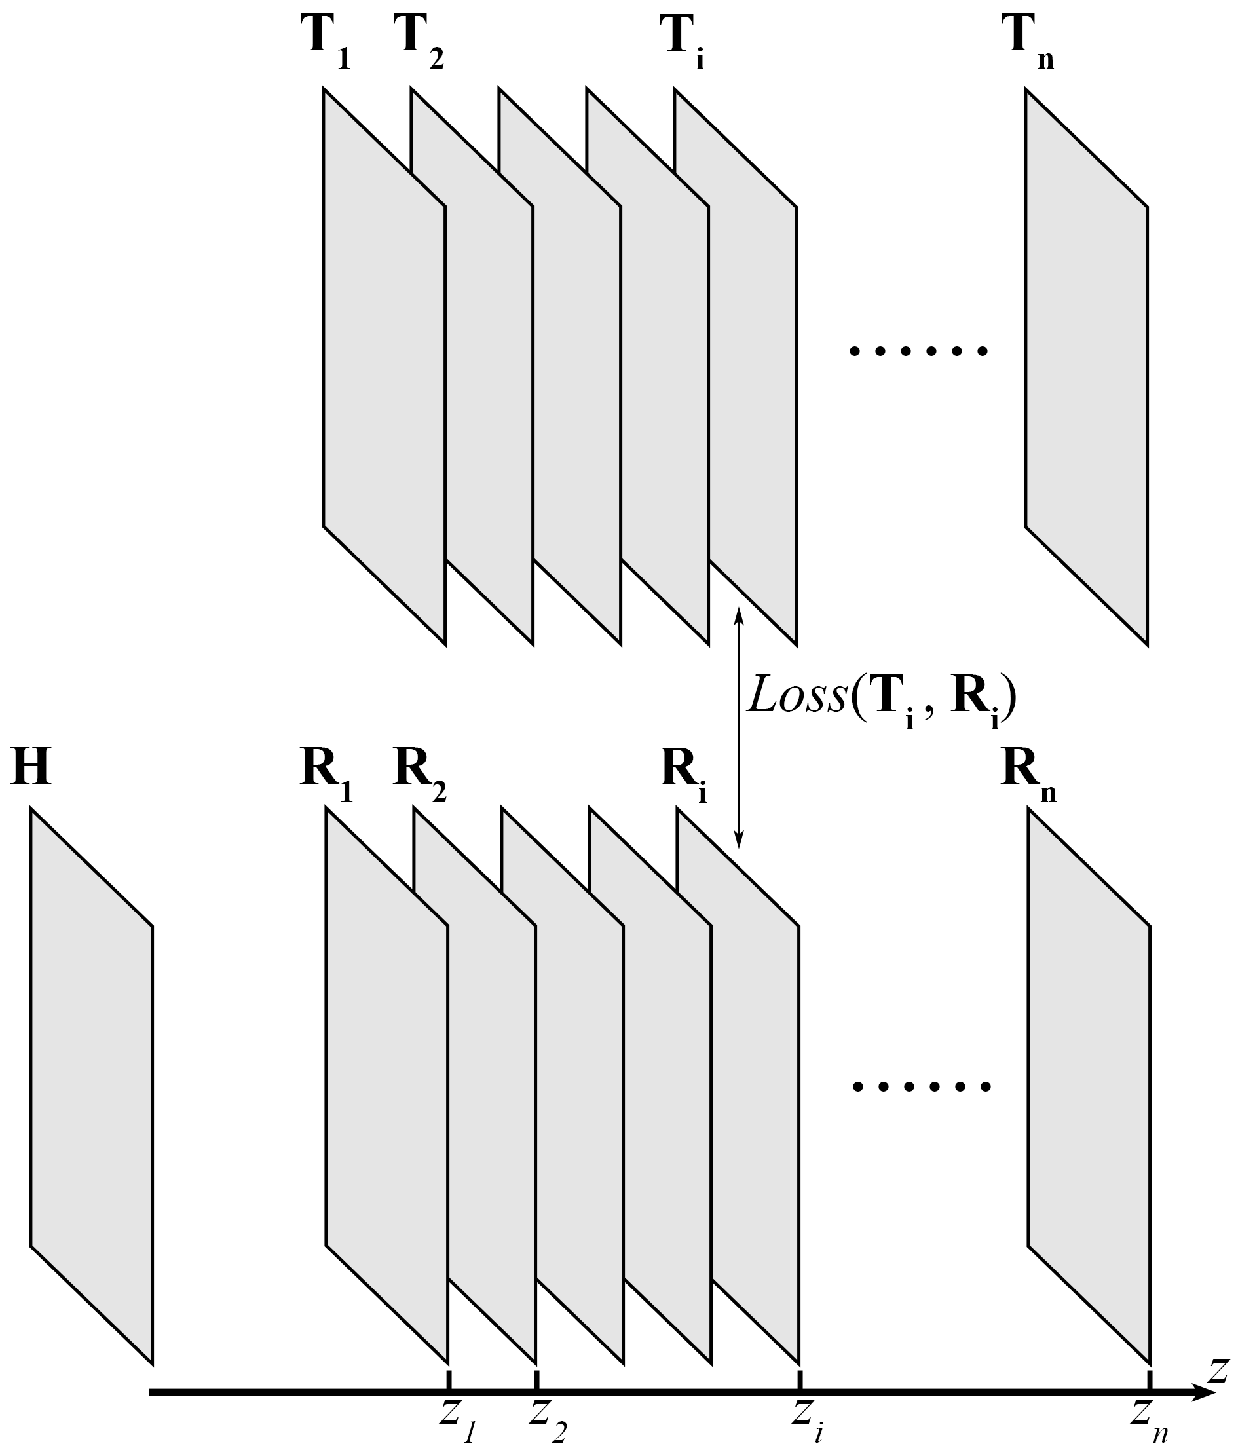
\includegraphics[width=0.5\textwidth]{Fresnel_slice_illustration}
	\caption{Loss between the multi-depth targets ($\textbf{T}_1$ to $\textbf{T}_n$) and the reconstructions ($\textbf{R}_1$ to $\textbf{R}_n$) of hologram $\textbf{H}$}
	\label{fig:Fresnel_slice_illustration}
\end{figure}

As shown in \cref{fig:Fresnel_slice_illustration}, the multi-depth target is set up as a collection of $n$ slices ($\textbf{T}_1$ to $\textbf{T}_n$), each slice $\textbf{T}_i$ is at a distance $z_i$ to the hologram plane. And for the hologram $\textbf{H}$, its reconstruction at each distance $z_i$ is computed using Fresnel diffraction formula in \cref{eq:fresnel-diffraction}, which is labelled as the propagation function $\mathcal{P}(\textbf{H}, z_i)$.

Then, to create an objective function ($f(\textbf{x})$ in \cref{eq:minimise_F}) to optimise, we need to quantify the difference between each target slice ($\textbf{T}_i$) and the respective reconstruction ($\textbf{R}_i$) numerically, and minimize such difference. Among the lots of options available, the loss functions selected are mean squared error (MSE) \cite{MSE_REF}, cross entropy (CE) \cite{cybenko1998mathematics} and relative entropy (RE) \cite{Kullback1951}. To adapt the loss functions for two-dimensional (2D) target image $\textbf{T}_i$ and reconstructed image $\textbf{R}_i$ of dimension $X\times Y$, the loss functions are adapted as shown in \cref{eq:MSE_holo} to \cref{eq:RE_holo}.

\begin{align}
	MSE(\textbf{T}_i, \textbf{R}_i) & = \frac{1}{X\times Y} \sum_{x=1}^{X} \sum_{y=1}^{Y} (\textbf{T}_{i;x,y}-\textbf{R}_{i;x,y})^2\label{eq:MSE_holo}                     \\
	CE(\textbf{T}_i, \textbf{R}_i)  & = -\sum_{x=1}^{X} \sum_{y=1}^{Y} \textbf{T}_{i;x,y}\log(\textbf{R}_{i;x,y})\label{eq:CE_holo}                                        \\
	RE(\textbf{T}_i, \textbf{R}_i)  & = -\sum_{x=1}^{X} \sum_{y=1}^{Y} \textbf{T}_{i;x,y}\log\left(\frac{\textbf{R}_{i;x,y}}{\textbf{T}_{i;x,y}}\right) \label{eq:RE_holo}
\end{align}

Mean squared error (MSE) is adapted as shown in \cref{eq:MSE_holo}. MSE is a traditional metric averaging the squared error between the target and observed values. Cross entropy (CE) is adapted as shown in \cref{eq:CE_holo}. CE is often used in classification problems, such as language modelling \cite{Liu2018}. Relative entropy (RE), also called Kullback-Leibler divergence (usually denoted as $D_{KL}(P\vert\vert Q)$), is adapted as shown in \cref{eq:RE_holo}. For the uniformity of symbols in this paper, relative entropy is denoted as RE. It is a measure of how much a probability distribution $P$ is different from another probability distribution $Q$. Both CE and RE are usually computed between the true probabilistic distribution and the predicted probabilistic distribution, while the images are not probability distributions, the pixel values are normalized to decimal numbers in the range of 0 to 1 so that CE and RE can be applied.

The effectiveness of L-BFGS optimisation of phase-only CGH for a single slice target image ($n=1$) has been demonstrated in the previous research \cite{Sha2022}. However, for a 3D target consisted of multiple slices at different depths, the optimisation of CGH becomes challenging.

The typical technique is to sum the losses computed for each slice for each iteration during optimisation, which is called the Sum-of-Loss (SoL) method in this paper. At every iteration, it computes the full 3D reconstructions ($\textbf{R}_1, \cdots, \textbf{R}_n$) of the hologram $\textbf{H}$ at every distance $z_i$, requiring a total of $n$ Fourier Transforms, and then computes the total loss between all the target slices and the reconstructed slices, therefore fully evaluating the hologram at each step. Although the total number of iterations does not scale with $n$, the number of Fourier Transforms performed at each iteration scales up with $n$, as it needs to compute the full multi-depth reconstructions at every iteration.
\begin{equation}
	\text{SoL:}\quad \underset{\textbf{H}}{\arg \min}\ \sum_{i = 1}^{n} Loss(\textbf{T}_i, \textbf{R}_i)
\end{equation}

Another universal technique for 3D CGH is to sum the sub-holograms $\textbf{H}_i$ generated for each target slice $\textbf{T}_i$ to form a total hologram based on the principle of superposition, which is called the Sum-of-Hologram (SoH) method in this paper. For a fixed number of iterations for each sub-hologram, the total computation scales up linearly with the number of slices $n$. SoH method's advantage is its ease of implementation, that it can compute multi-depth 3D CGH based on any existing single slice CGH algorithm. Its major disadvantage for phase-only hologram generation is that, the final summing of sub-holograms will result in a non-uniform amplitude hologram, and taking the phase of which will result in discarding the amplitude information of the summed hologram, leading to worse reconstructions quality. And also, SoH method suffers from the defocusing effect from one slice to another, causing additional noise.
\begin{equation}
	\text{SoH:}\quad \sum_{i = 1}^{n} \underset{\textbf{H}_i}{\arg \min}\ Loss(\textbf{T}_i, \textbf{R}_i)
\end{equation}

\begin{figure}[h!]
	\centering
	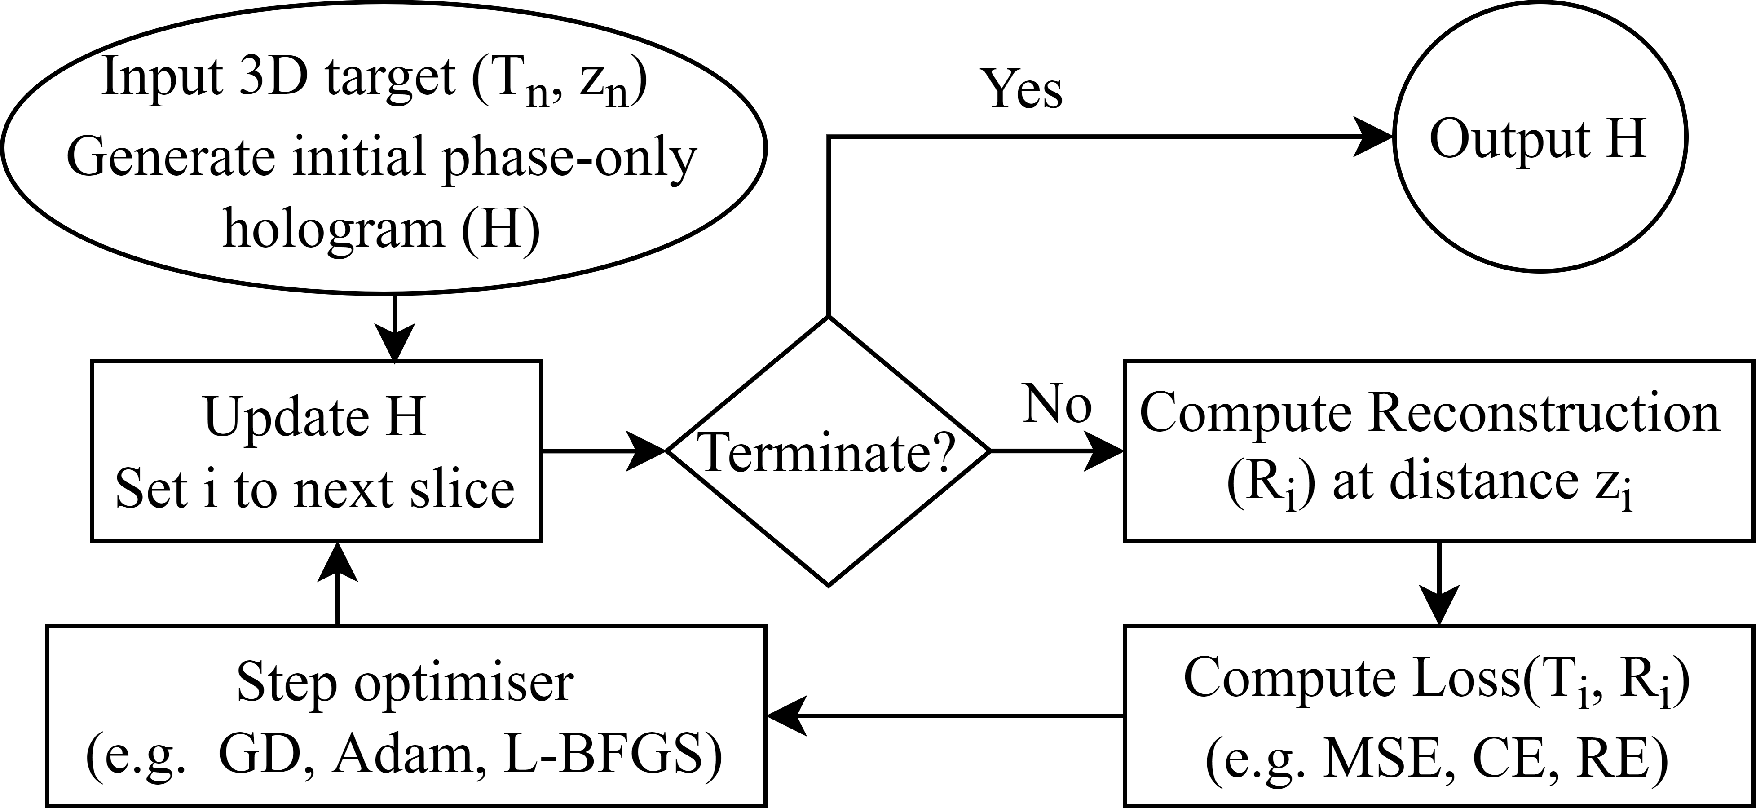
\includegraphics[width=0.8\textwidth]{optim3d-cgh-flowchart}
	\caption{Optimisation of CGH with sequential slicing (SS) flowchart}
	\label{fig:optim3d-cgh-flowchart}
\end{figure}

This paper proposes a novel CGH optimisation with sequential slicing (SS) technique, as shown in the flowchart in \cref{fig:optim3d-cgh-flowchart}, that only computes the loss for a single slice at each iteration (between a reconstruction $\textbf{R}_i$ at a single distance $z_i$ and its according target slice $\textbf{T}_i$), where $i$ sweeps through the multi-layer 3D target sequentially when the algorithm iterates. When the final slice is reached ($i=n$), it goes back to the first slice ($i \gets 1$). The proposed method only needs to carry out one Fourier Transform at each iteration, and the number of iterations does not need to scale up with $n$. So it is expected to be much quicker than SoL and SoH techniques while producing proper resulting hologram.










%%%%%%%%%%%%%%%%%%%%%%%%%%  Results  %%%%%%%%%%%%%%%%%%%%%%%%%%
\section{Results}
\subsection{CGH for 4-slice targets}

\begin{figure}[h!]
	\centering
	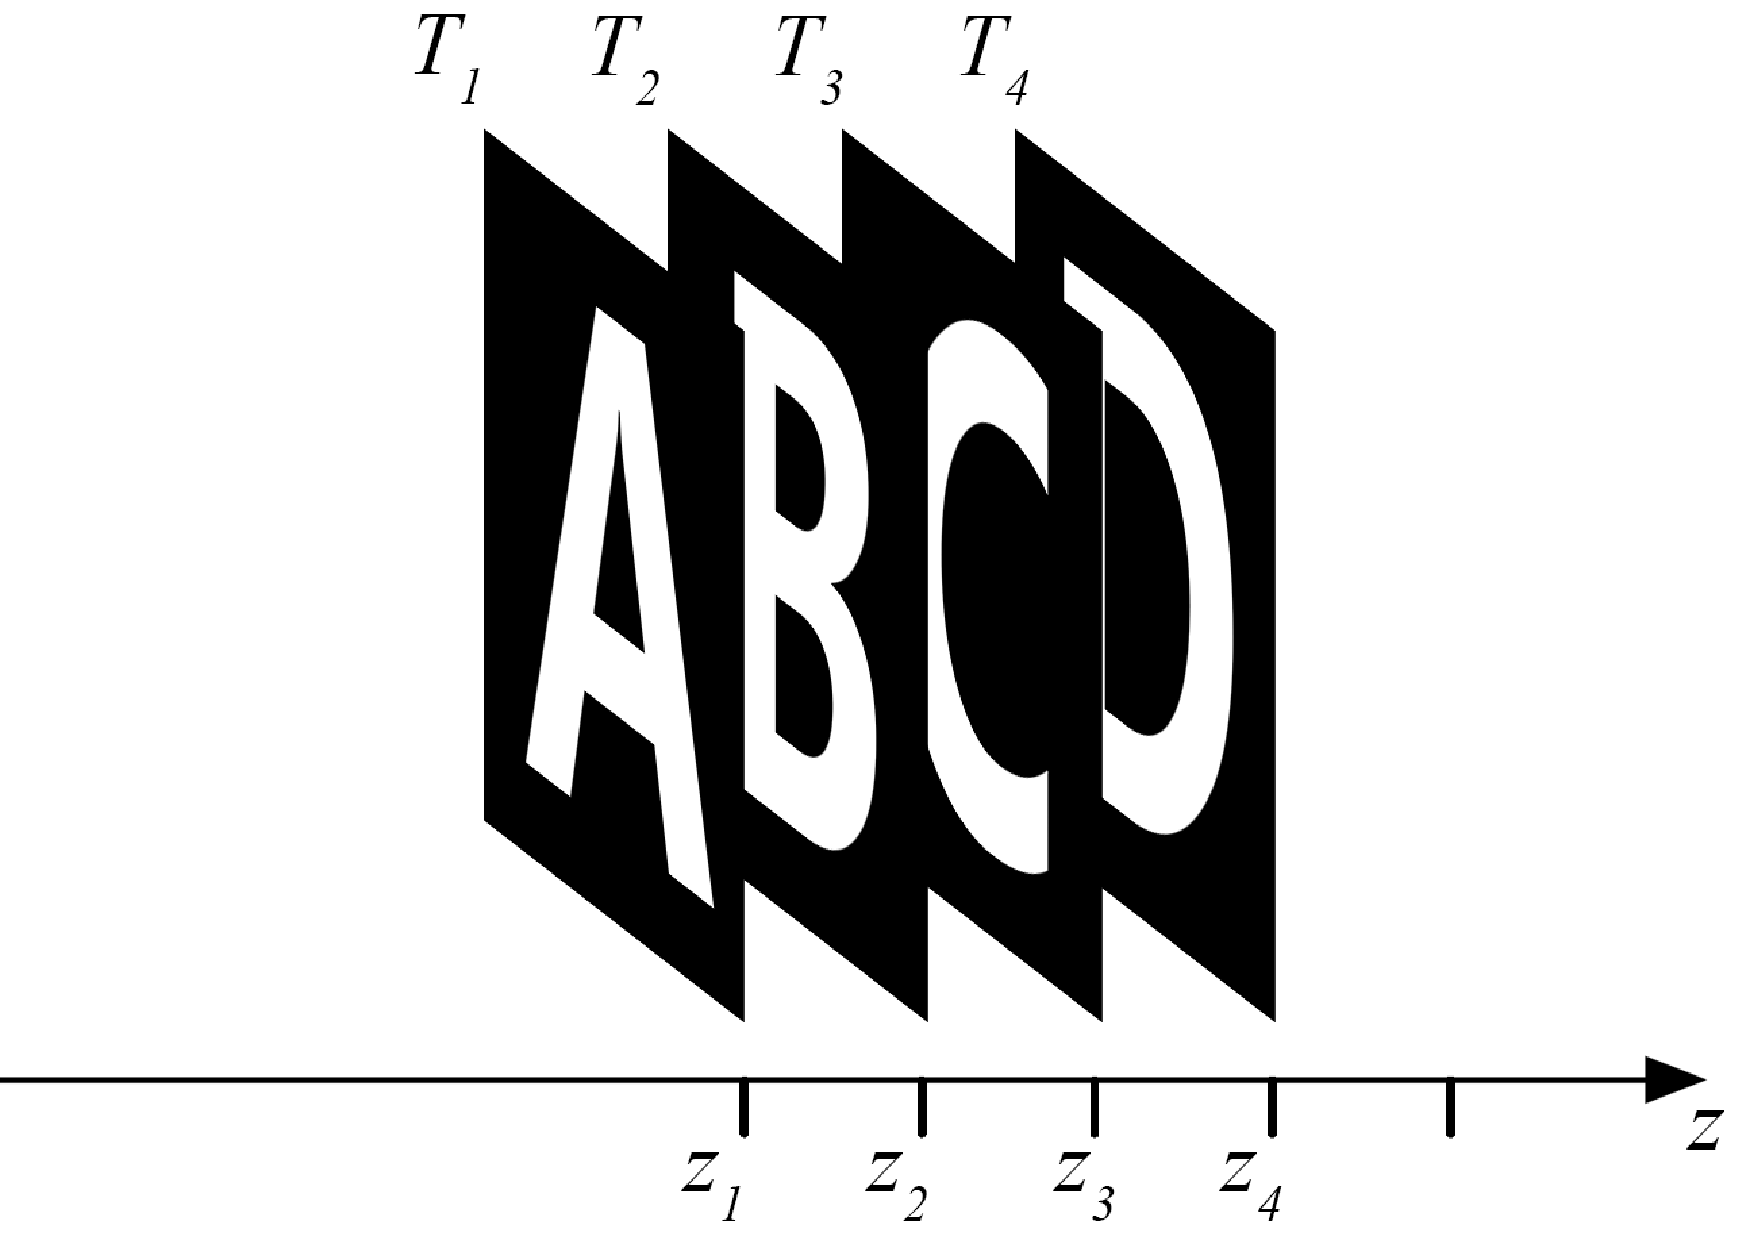
\includegraphics[width=0.5\textwidth]{Fresnel_slice_ABCD}
	\caption{Layout of the 4-slice target ($z_1=1\ cm$, $z_2=2\ cm$, $z_3=3\ cm$, $z_4=4\ cm$)}
	\label{fig:Fresnel_slice_ABCD}
\end{figure}

The first example 3D target used is consisted of 4 slices made from alphabets `A', `B', `C', `D', each has $512\times512$ pixels. The positions of the four slices range from $1\ cm$ to $4\ cm$ with $1\ cm$ gap between each other (i.e. $z_i=i\ cm$). The overall layout is shown in \cref{fig:Fresnel_slice_ABCD}.

As there are two optimisation algorithms (GD and L-BFGS), three techniques (SoL, SoH and SS) and three loss functions (MSE, CE, RE) in consideration, they can form a total of 18 combinations. In order to control the number of variables, all 18 combinations are set to start from the same initial random hologram and run for the same amount of 100 iterations for the optimisation of each hologram, on the same laptop of model ASUS ROG Zephyrus M16, which has a CPU of model i7-11800H and a GPU of model RTX3060. For the L-BFGS algorithm, the gradient history of size 10 ($m=10$ in \cref{alg:L-BFGS}) is used for all techniques and loss functions. And to ensure a sensible comparison, although three different loss functions are used for optimisation of CGH, the metric used to assess the quality of multi-depth reconstructions of the final hologram is the normalized mean squared error (NMSE). As there are a total of 4 slices in this example, the final NMSE of each are computed separately and the total optimisation run time is recorded. The final results are gathered in \cref{fig:Technique_Loss_comparison}. As each slice has a different final error, their mean and standard deviation (SD) are computed for investigations. Three columns are colour coded where green indicates better result while red indicates worse result.

\begin{figure}[h!]
	\centering
	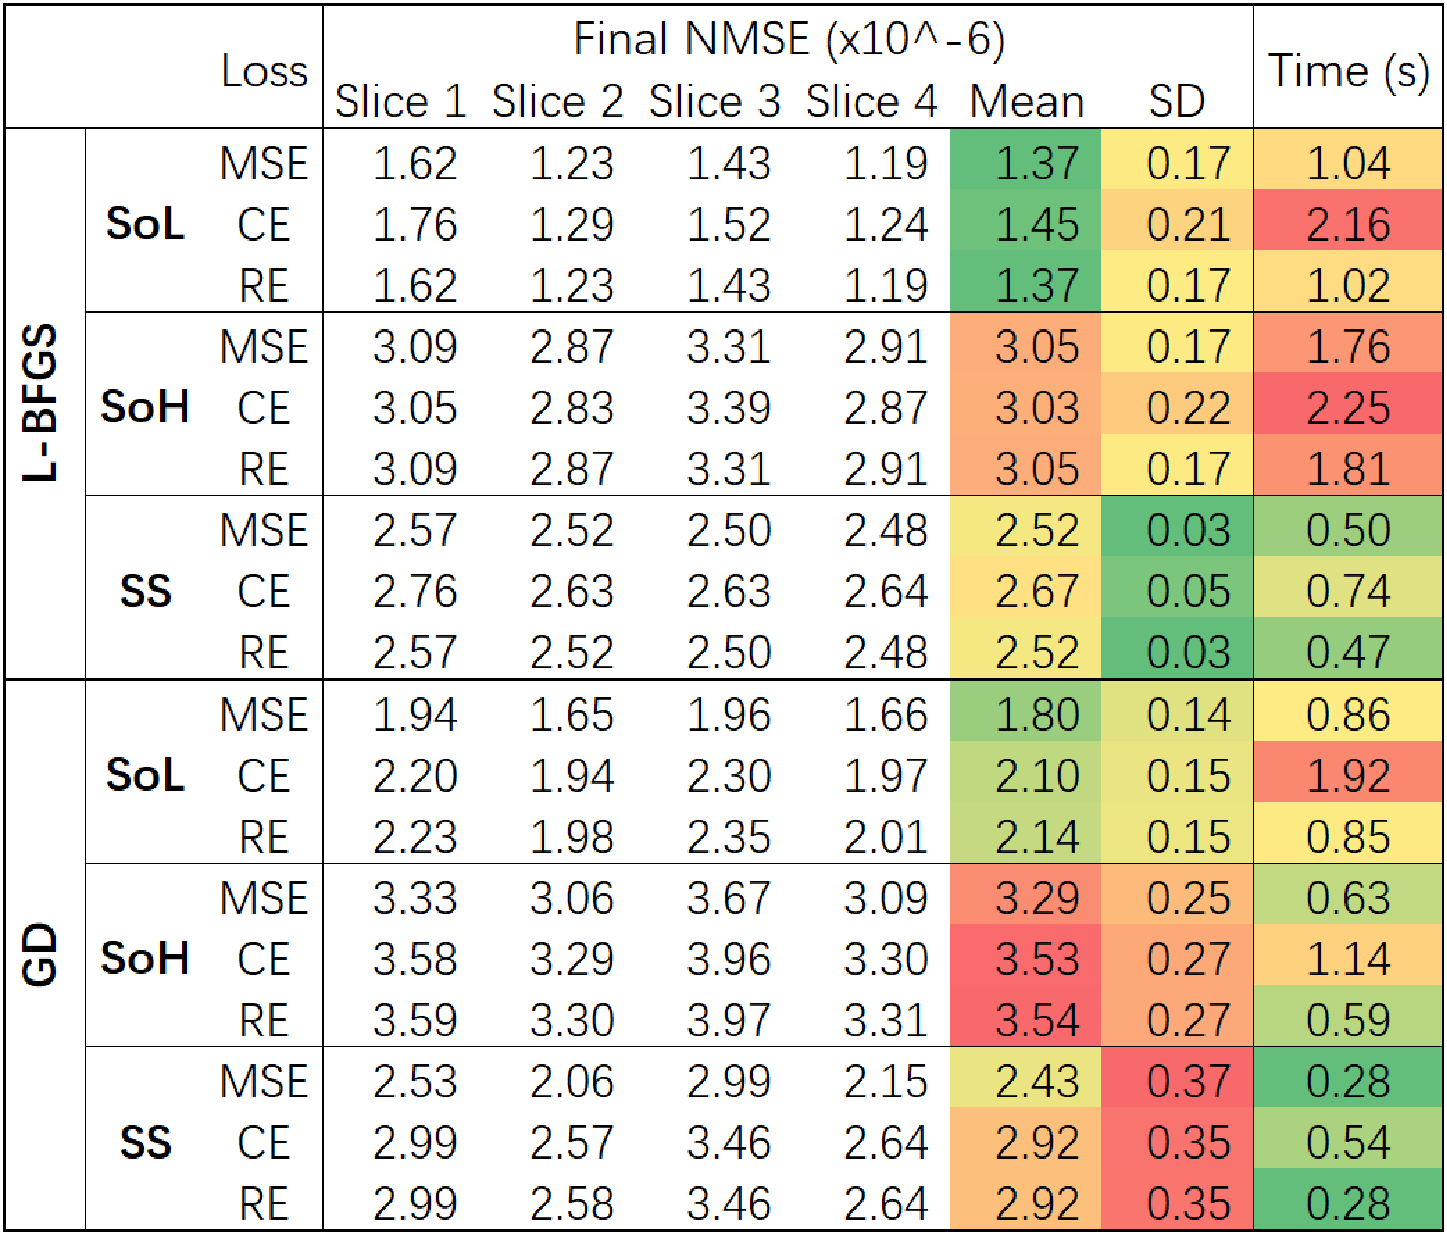
\includegraphics[width=0.5\textwidth]{Technique_Loss_comparison}
	\caption{Final NMSE and run time comparison across the three techniques}
	\label{fig:Technique_Loss_comparison}
\end{figure}

Comparing the mean of final NMSE and the run time of the proposed sequential slicing (SS) technique to those of the sum-of-loss (SoL) and sum-of-hologram (SoH) techniques in \cref{fig:Technique_Loss_comparison}, it can be concluded that, for all combinations of optimisers and loss functions attempted, the proposed SS technique runs much quicker than the existing SoL and SoH techniques, while still providing a proper result, sitting between the SoL and SoH techniques. So the SS technique has not demonstrated absolute advantage to the SoL technique yet on this 4-slice example, therefore further investigation is done on a 30-slice example in \cref{sec:30-slice-target}. However, the SS technique is both quicker and has better reconstructions quality than the SoH technique, demonstrating an absolute advantage. Meanwhile, the combinations with CE as loss function are much slower and has not demonstrated advantage in average NMSE, demonstrating an absolute disadvantage, so the results with CE loss or SoH method will not be shown in the per-iteration plots.

\begin{figure}[h!]
	\centering
	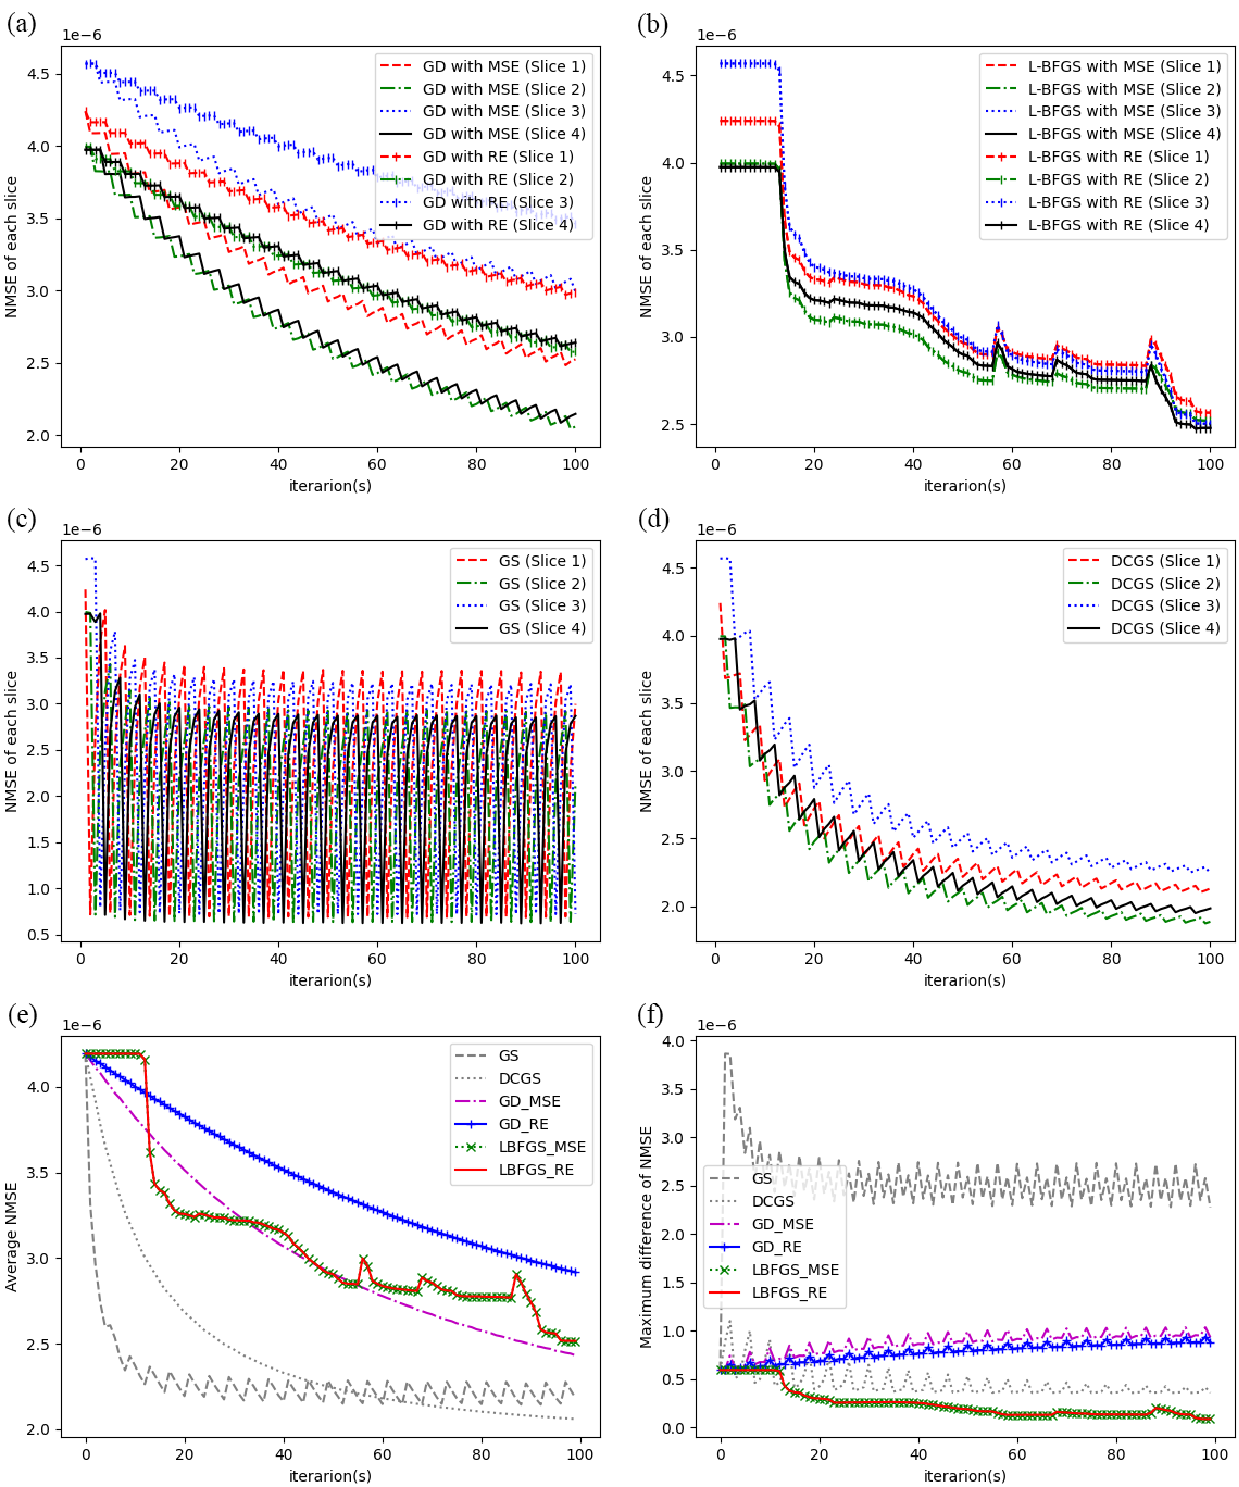
\includegraphics[width=1.0\textwidth]{Comparison_among_SS_methods_for_the_4_slice_target}
	\caption{Comparison among SS techniques for the 4-slice target using (a) GD algorithm, (b) L-BFGS algorithm, (c) GS algorithm, (d) DCGS algorithm. (e) Average NMSE, and (f) difference between the maximum and minimum NMSE across all slices.}
	\label{fig:SS_NMSE_iteration_compare}
\end{figure}
For comparison among the sequential slicing (SS) techniques, the NMSE for each slice and their average and maximum difference values are plotted for GD and LBFGS algorithms with MSE and RE loss functions in \cref{fig:SS_NMSE_iteration_compare}, and sequential GS and DCGS \cite{Zhou2019} are also implemented and plotted for reference purpose. Apart from the L-BFGS algorithm, all the other algorithms are showing a staircase-like plot, where a decrease in error on one slice results in an increase in error on all other slices, and so the final NMSE of each slice distinguishes a lot from each other. The sequential GS algorithm suffers the most from the quality imbalance between each slice, and the sequential GD algorithm follows. The DCGS algorithm benefits from its modification of the inclusion of a weighting factor consisting historical amplitude, therefore managed to converge. From the average NMSE plot (\cref{fig:SS_NMSE_iteration_compare} (e)), the proposed sequential L-BFGS method does not appear to have the lowest average NMSE, but it has the lowest quality imbalance across the slices as shown in the maximum difference plot (\cref{fig:SS_NMSE_iteration_compare} (f)). The L-BFGS algorithm mainly benefits from its inclusion of curvature information during optimisation, so that the update of hologram $\textbf{H}$ at each iteration takes into account not only the loss for current slice, but also all historical iterations up to the set history size ($m$ in \cref{alg:L-BFGS}). So the NMSE of each slice stays close for L-BFGS and at each iteration, the NMSE of all slices behave in the same way, ensuring each slice to have the similar quality.


\begin{figure}[h!]
	\centering
	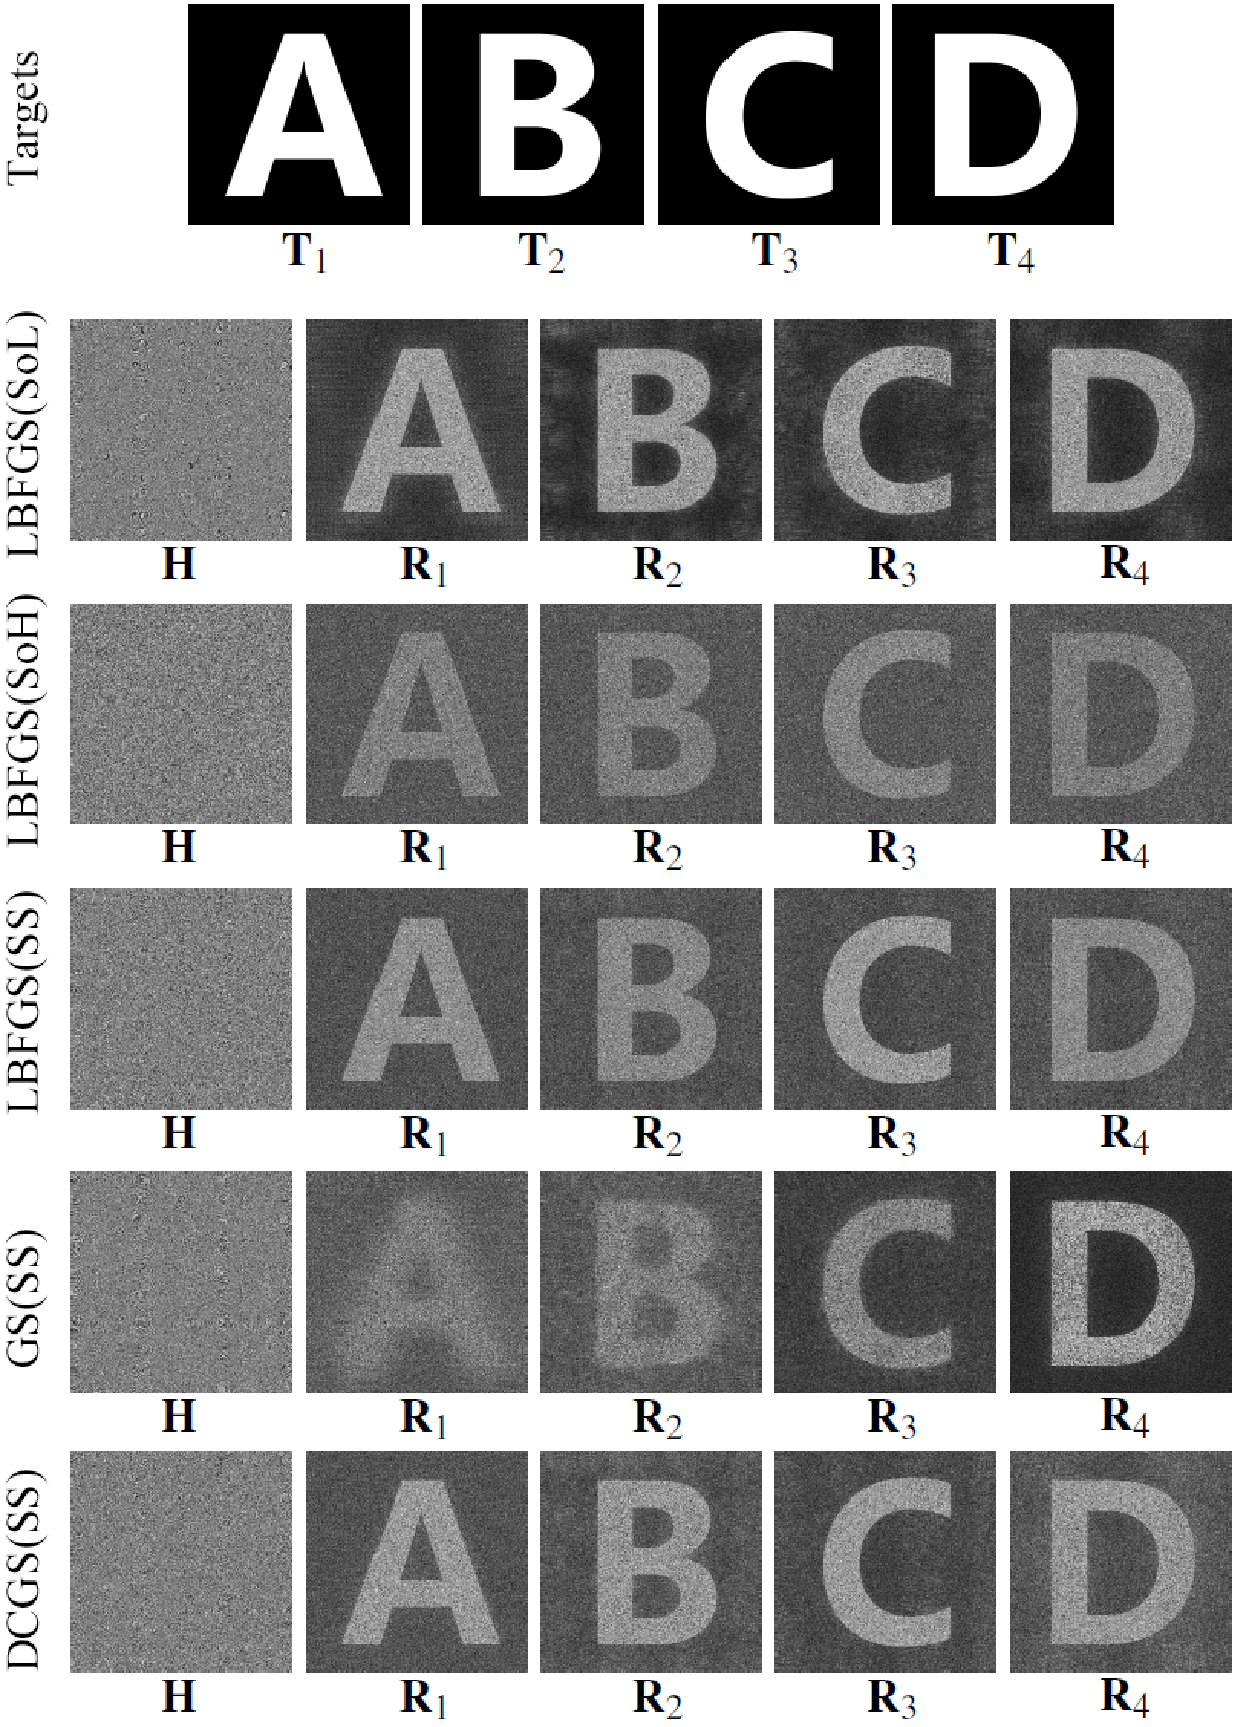
\includegraphics[width=0.5\textwidth]{final_holograms_reconstructions_4_slice}
	\caption{Comparison of final holograms and reconstructions}
	\label{fig:3D_ABCD}
\end{figure}

The final holograms and their reconstructions for L-BFGS algorithm with SoL, SoH and SS techniques are shown in \cref{fig:3D_ABCD}, with GS with SS technique and DCGS also shown as reference. The reconstructed images confirm the SS technique having a quality between SoH and SoL method (for the same amount of iterations), and has a much better quality imbalance than sequential GS, which has a very clear reconstruction at the fourth slice (letter `D') because the iteration stopped at the fourth slice but much worse reconstructions at other slices. Admittedly, the proposed L-BFGS with SS method cannot surpass the GS-based DCGS algorithm yet.




\begin{figure}[h!]
	\centering
	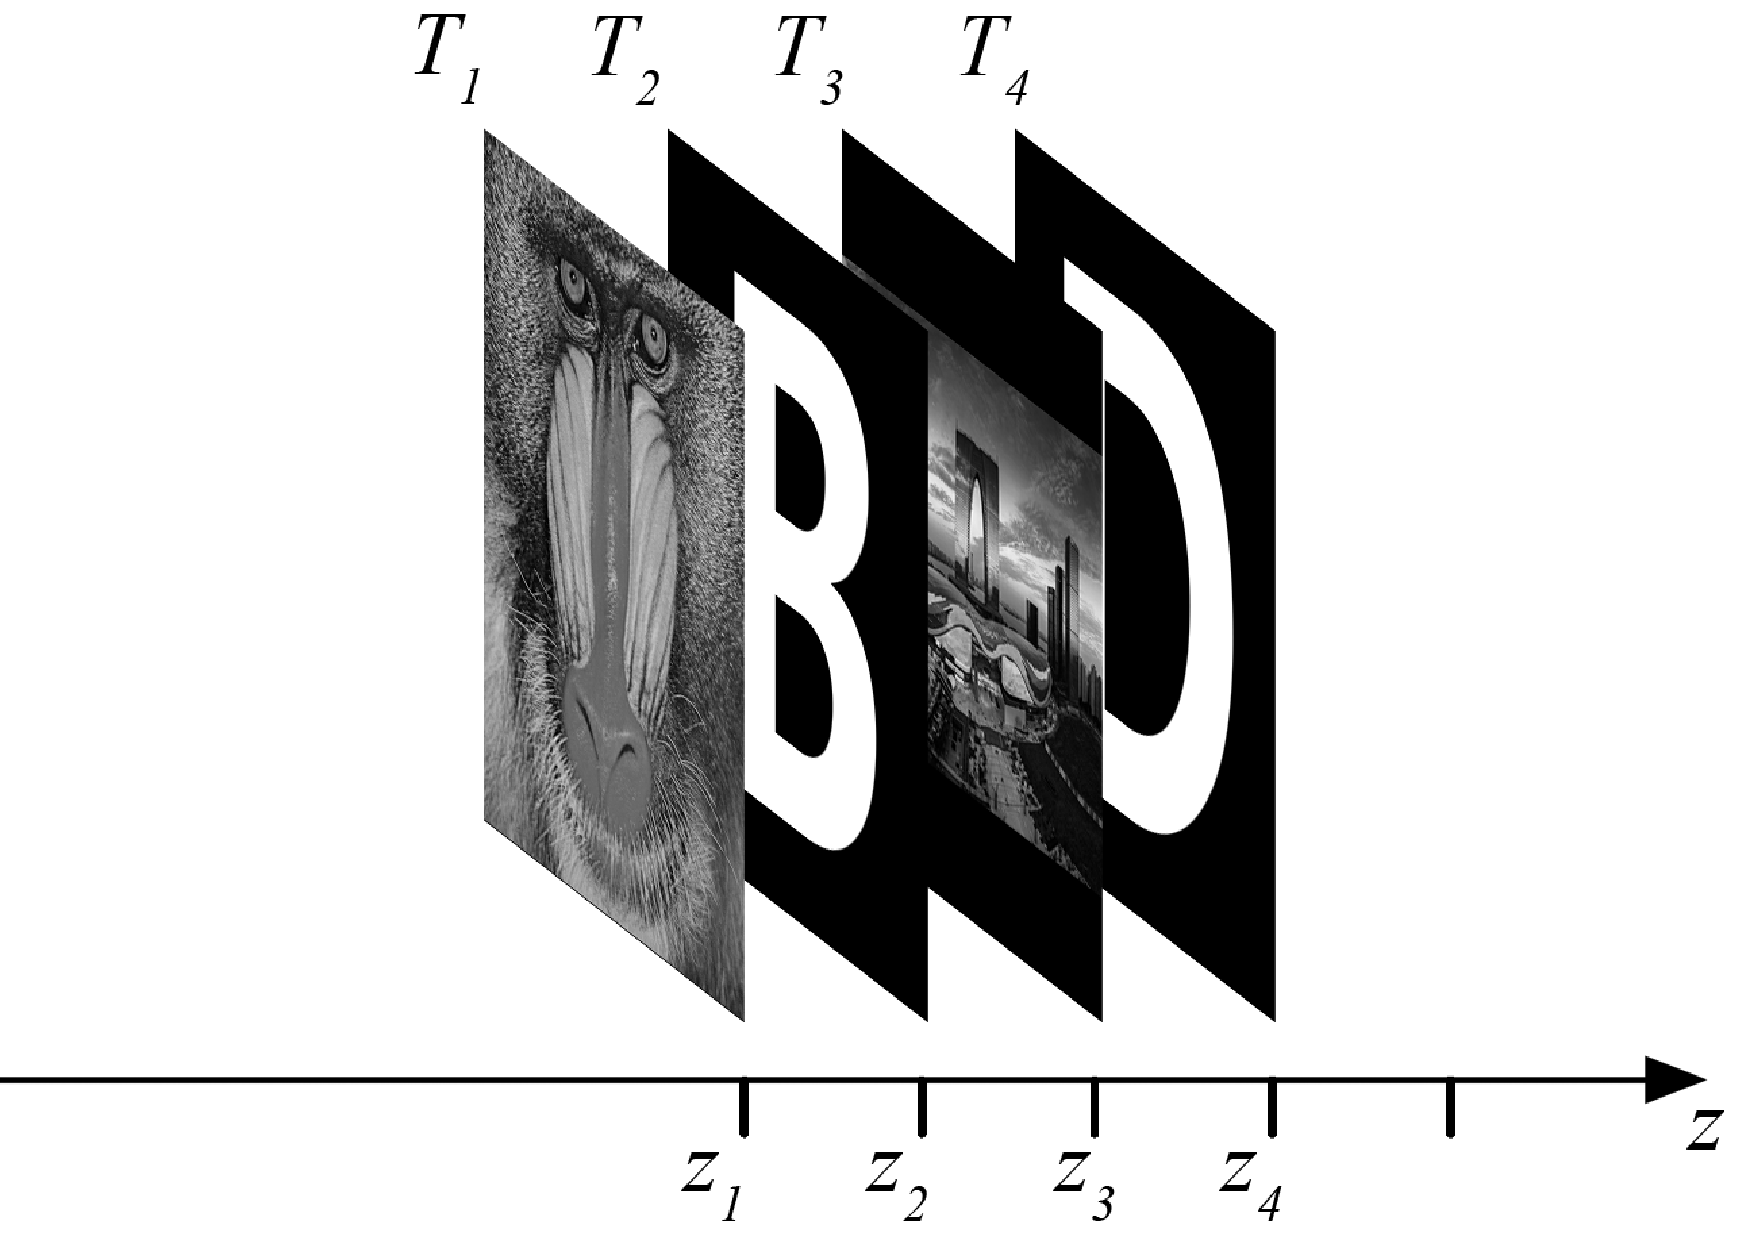
\includegraphics[width=0.5\textwidth]{Fresnel_slice_mandrill_B_szzx_D}
	\caption{Layout of the non-binary 4-slice target}
	\label{fig:more_difficult_3d_target_layout}
\end{figure}

To prove that the proposed method also works for non-binary targets, another example of a 4-slice 3D target was attempted, as shown in \cref{fig:more_difficult_3d_target_layout}, where two of the slices are replaced by an image of the mandrill \cite{MANDRILL_REF} and an image of the city scene \cite{Zhang2017} respectively.

\begin{figure}[h!]
	\centering
	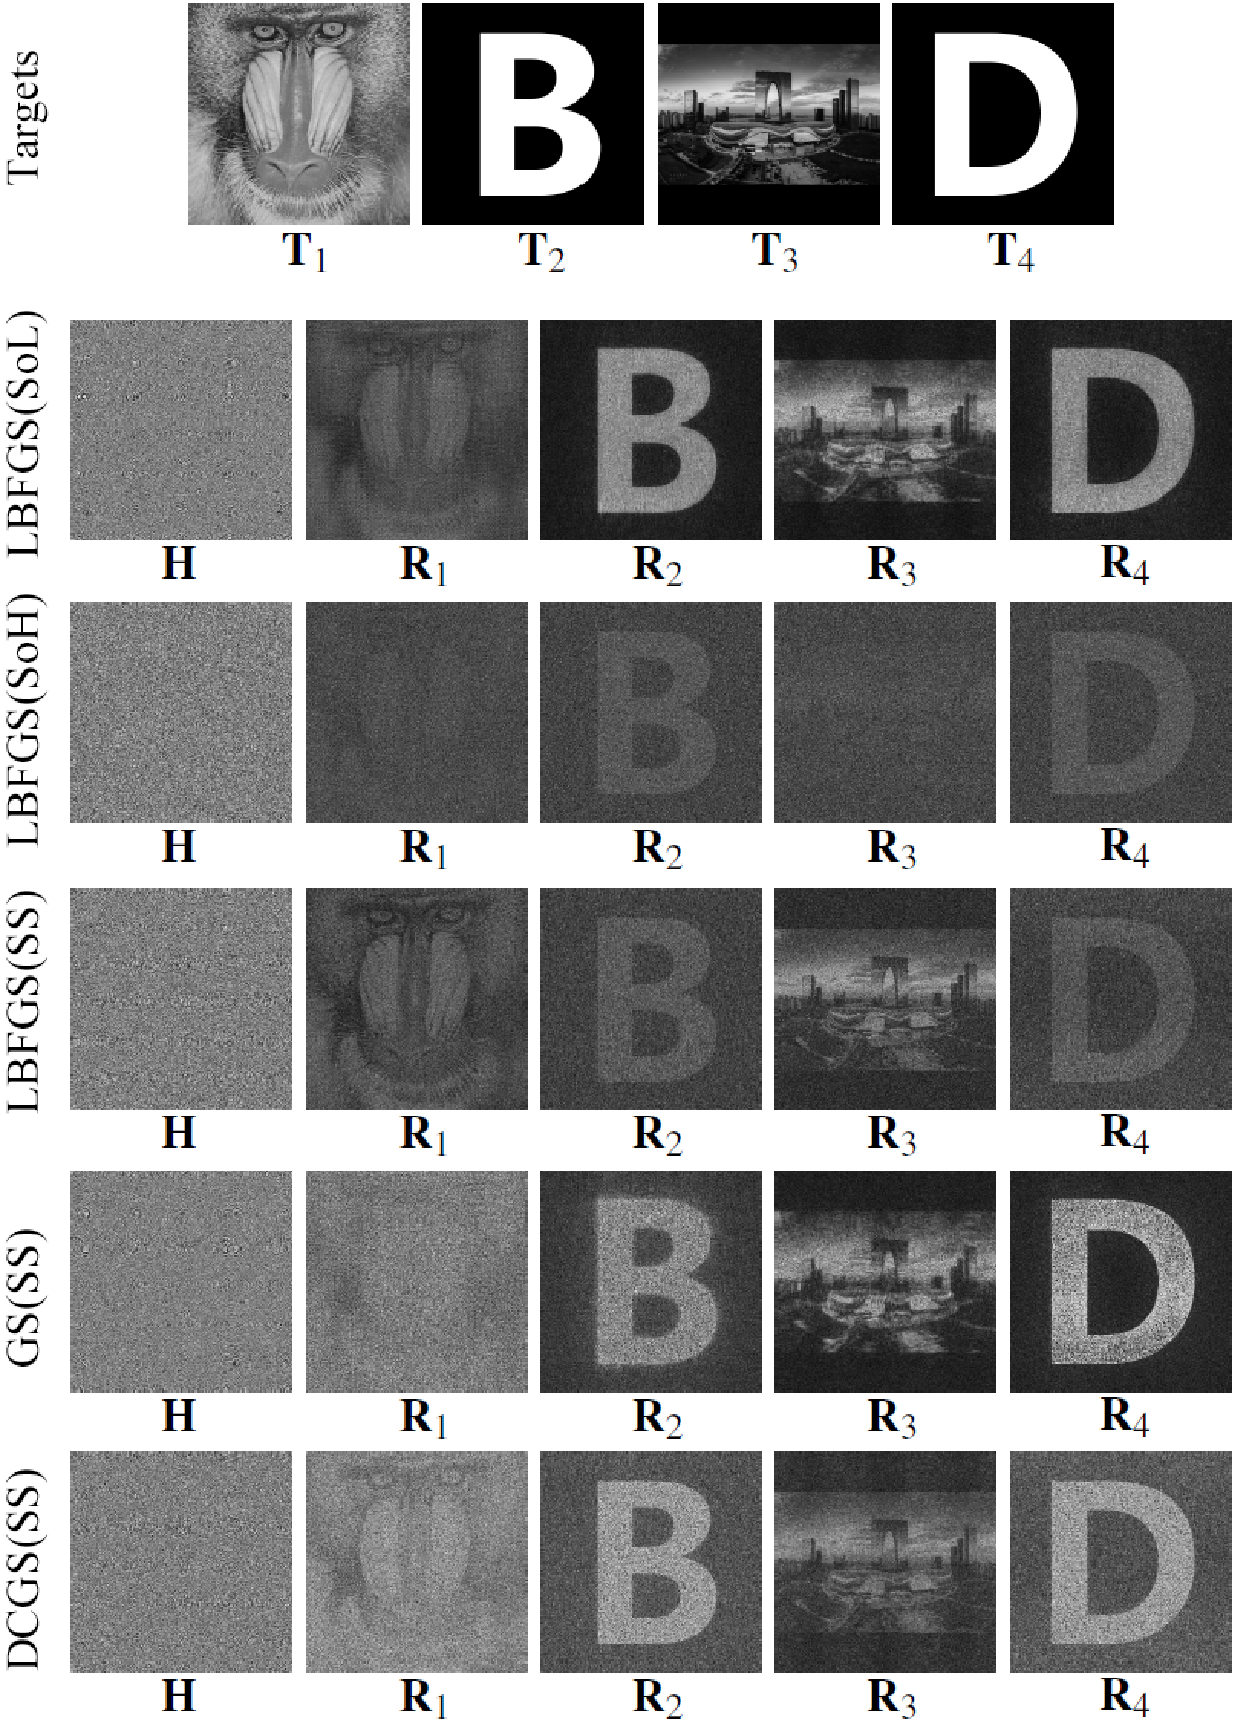
\includegraphics[width=0.5\textwidth]{final_holograms_reconstructions_4_slice_non_binary}
	\caption{Comparison of final holograms and reconstructions for non-binary target}
	\label{fig:more_difficult_3d_target_recon}
\end{figure}

As shown in the final holograms and reconstructions in \cref{fig:more_difficult_3d_target_recon}, the proposed LBFGS with SS technique still managed to converge, with final reconstructions quality sitting between the SoL and SoH method, and also having a good quality balance across all slices.



\newpage
\subsection{CGH for a 30-Slice Target} \label{sec:30-slice-target}

\begin{figure}[h!]
	\centering
	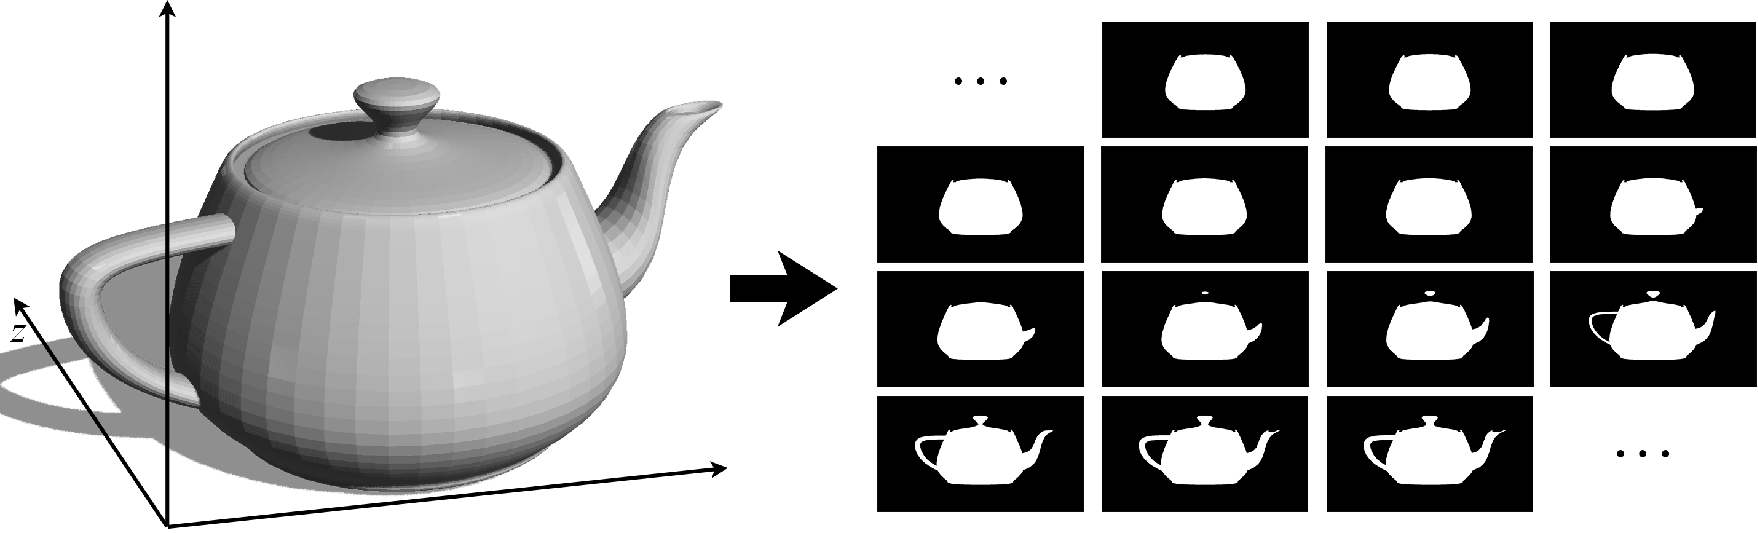
\includegraphics[width=0.5\textwidth]{Utah_teapot_target}
	\caption{30-slice target sliced from a 3D Teapot mesh}
	\label{fig:Teapot_target}
\end{figure}

Another example of a 30-slice target sliced from a 3D teapot is attempted for speed analysis when the number of slices go higher. As shown in \cref{fig:Teapot_target}, the Utah teapot \cite{Clark2015} is sliced into 30 planes, each of 720p resolution ($1280\times720$). Each combination in \cref{fig:Technique_Loss_comparison} were run on a laptop of model ASUS ROG Zephyrus M16 with a CPU of model i7-11800H and a GPU of model RTX3060. The average and maximum difference of NMSE across all slices plotted against time (in \cref{fig:Teapot_Average_NMSE_vs_time} and \cref{fig:Teapot_Max_diff_NMSE_vs_time} respectively) for all combinations except those with SoH technique or with CE as loss function as they have absolute disadvantage, for clearer plots.

\begin{figure}[h!]
	\centering
	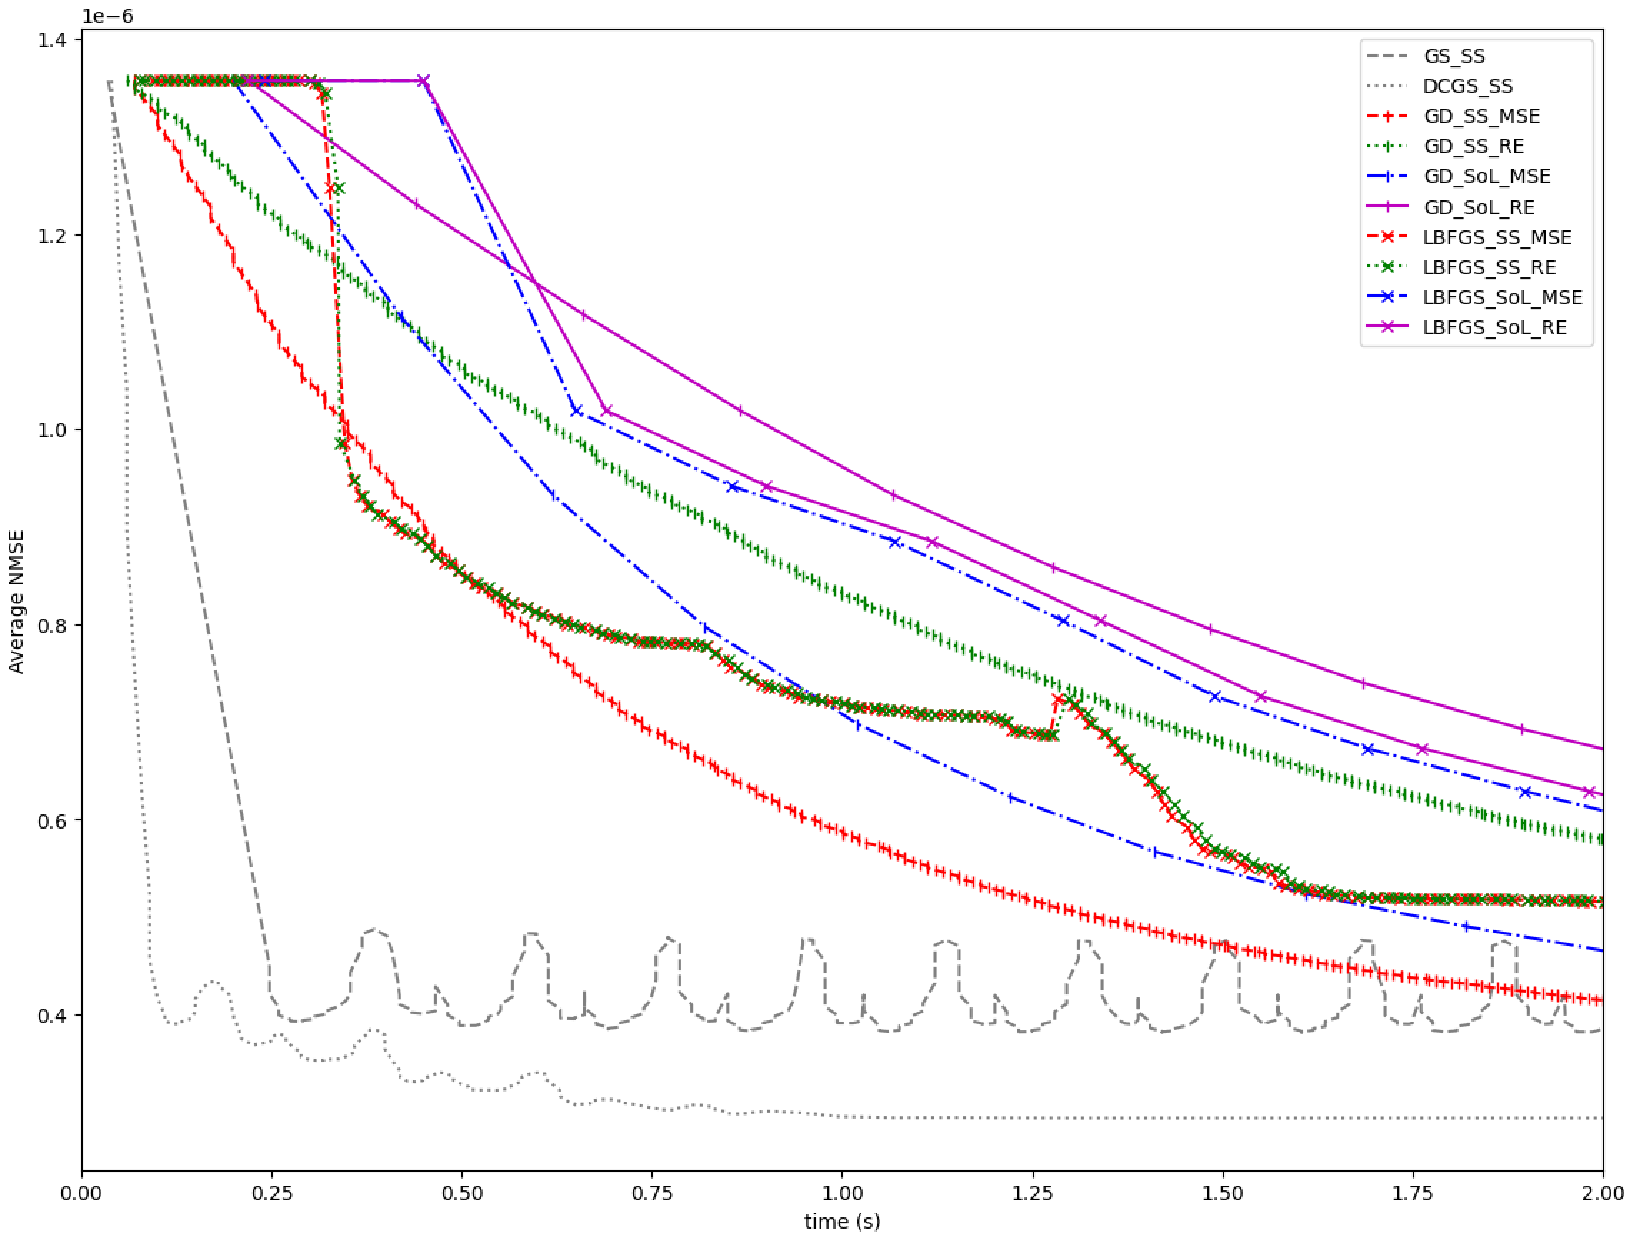
\includegraphics[width=1.0\textwidth]{Teapot_Average_NMSE_vs_time}
	\caption{Average NMSE v.s. time plot for the 30-slice target}
	\label{fig:Teapot_Average_NMSE_vs_time}
\end{figure}

\begin{figure}[h!]
	\centering
	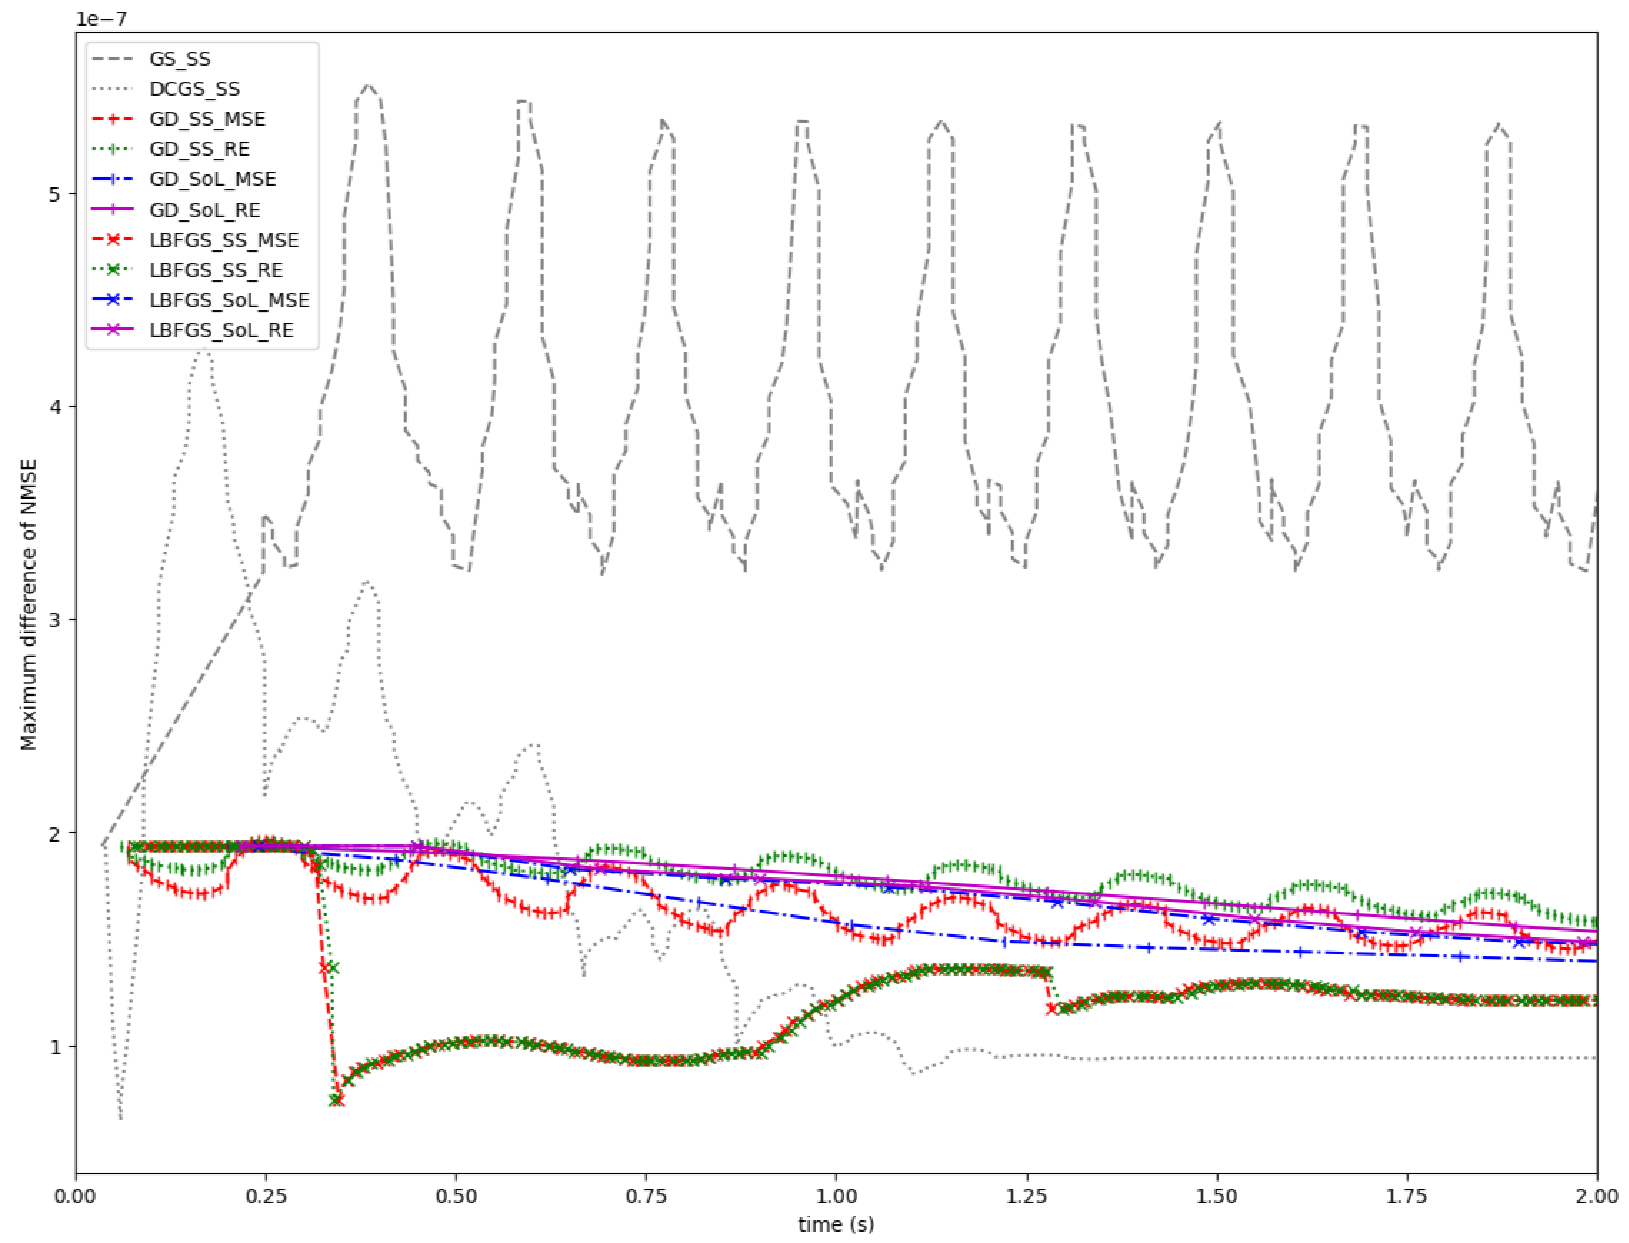
\includegraphics[width=1.0\textwidth]{Teapot_Max_diff_NMSE_vs_time}
	\caption{Difference between the maximum and minimum NMSE across all slices v.s. time plot for the 30-slice target}
	\label{fig:Teapot_Max_diff_NMSE_vs_time}
\end{figure}

\cref{fig:Teapot_Average_NMSE_vs_time} shows that, for both GD and L-BFGS optimisation algorithms, the SS technique is faster than the SoL technique. Among the SS techniques, GD, GS and DCGS algorithms achieved less average NMSE than the proposed L-BFGS with SS method, but from the maximum difference of NMSE plot in \cref{fig:Teapot_Max_diff_NMSE_vs_time}, it can be shown that the L-BFGS algorithm has less quality imbalance than the GD algorithm and the GS algorithm, although admittedly it is not as good as the DCGS algorithm. Nevertheless, the proposed method has achieved an improvement of phase retrieval using optimisation algorithms, in speed and quality imbalance suppression.


%%%%%%%%%%%%%%%%%%%%%%%%%%  Conclusion  %%%%%%%%%%%%%%%%%%%%%%%%%%
\section{Conclusion}
This paper has proposed the method of using L-BFGS optimisation algorithm to generate phase-only hologram for multi-depth target, and discussed its suitability with the sequential slicing (SS) technique. The L-BFGS with SS method has demonstrated a good suppression on the quality imbalance across the multi-depth slices, benefiting from the nature of being a second order optimisation algorithm, which implicitly records the historical gradients by other slices for the determination of the descent direction. For both GD and L-BFGS optimisation algorithms, the SS technique ran faster and produced better reconstruction quality than the simple SoH technique, and it is quicker than the SoH technique when the number of depths get large. The proposed method has demonstrated great potential of time constrained optimisation of multi-depth CGH.